\documentclass[12pt, twoside]{article}
\usepackage[francais]{babel}
\usepackage[T1]{fontenc}
\usepackage[latin1]{inputenc}
\usepackage[left=5mm, right=5mm, top=3mm, bottom=3mm]{geometry}
\usepackage{float}
\usepackage{graphicx}
\usepackage{array}
\usepackage{multirow}
\usepackage{amsmath,amssymb,mathrsfs}
\usepackage{soul}
\usepackage{textcomp}
\usepackage{eurosym}
 \usepackage{variations}
\usepackage{tabvar}


\pagestyle{empty}

\begin{document}


\section*{\center{Devoir maison 1}}

\medskip




\begin{center}
\fbox{

\textit{Devoir � rendre sur feuille grand format pour le
\textbf{mardi 16 octobre 2012}.}

}
\end{center}

\enskip


 \textit{\ul{Remarques:} La justification et la r�daction seront compt�es dans
 le bar�me. Un calcul non justifi� donnera 0 point. Vous pouvez trouver des
 rappels sur votre manuel p 257 � 266.}


\enskip

\ul{Exercice 1}: (\textit{3 points})

\enskip

On donne les expressions suivantes: $ A= \dfrac{2}{3} \div \dfrac{5}{6} -
\dfrac{2}{5}$ \quad et \quad $B= \dfrac{21 \times 10^{-3} \times 16 \times
10^7}{12 \times 10^2}$

\begin{enumerate}
  \item Ecrire A sous la forme d'une fraction irr�ductible en �crivant les
  diff�rentes �tapes du calcul.
  \item Donner l'�criture d�cimale de B puis son �criture scientifique (�crire
  les diff�rentes �tapes du calcul).
\end{enumerate}


\bigskip

\ul{Exercice 2}: (\textit{4 points})

\begin{tabular}{cc}
\begin{minipage}{12cm}
Construire un agrandissement de rapport $\dfrac{11}{5}$ de la figure ci-contre.

Expliquer votre d�marche.

L'unit� de longueur est le centim�tre.
\end{minipage}
&
\begin{minipage}{6cm}
\begin{center}
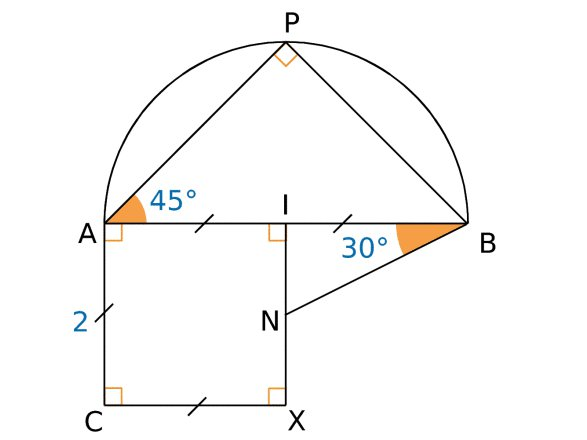
\includegraphics[width=5cm]{images/ex2.jpg} 
\end{center}
\end{minipage}
\end{tabular}

\bigskip

\ul{Exercice 3}: (\textit{7 points})

\enskip

\begin{tabular}{cc}
\begin{minipage}{15cm}

($\mathcal{C}$) est un cercle de centre E dont le diam�tre [AD] mesure 11 cm. B
est un point du cercle v�rifiant $\widehat{AEB}=48$�.

\begin{enumerate}
  \item Faire la figure en vraie grandeur.
  \item Montrer que le triangle ABD est rectangle.
  \item Calculer BE. En d�duire la nature du triangle AEB.
  \item Montrer que $\widehat{EAB}$=66�. En d�duire $\widehat{ADB}$.
  \item Calculer AB. On donnera une valeur arrondie au centi�me de centim�tre.
  \item On trace la droite parall�le � (AB) passant par E. Elle
  coupe le segment [BD] au point F. 
Compl�ter la figure.   
\item Calculer EF. On donnera une valeur arrondie au dixi�me de
  centim�tre.
 
\end{enumerate}
\end{minipage}
&
\begin{minipage}{4cm}
\begin{center}
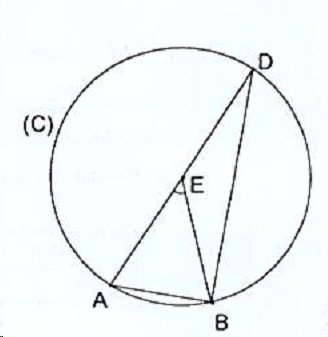
\includegraphics[width=4cm]{images/ex3.jpg} 
\end{center}
\end{minipage}

\end{tabular}

\bigskip

\ul{Exercice 4}: (\textit{7 points})


\enskip

\begin{tabular}{cc}
\begin{minipage}{15cm}

\begin{enumerate}

 \item Calculer DU. Justifier votre r�ponse.
 \item Calculer cos($\widehat{RDU}$) et cos($\widehat{REC}$). Que peut-on en
 d�duire pour les angles $\widehat{RDU}$ et $\widehat{REC}$?
 \item D�montrer que les droites (EC) et (DU) sont parall�les.
 \item Calculer le coefficient de r�duction premettant de passer du triangle
 RDU au triangle REC.
 \item Calculer le p�rim�tre des triangles RDU et REC. 
 \item Montrer que l'aire du triangle REC est �gale � 0,64 fois l'aire du
 triangle RDU.
\end{enumerate} 
\end{minipage}
&
\begin{minipage}{5cm}
\begin{center}
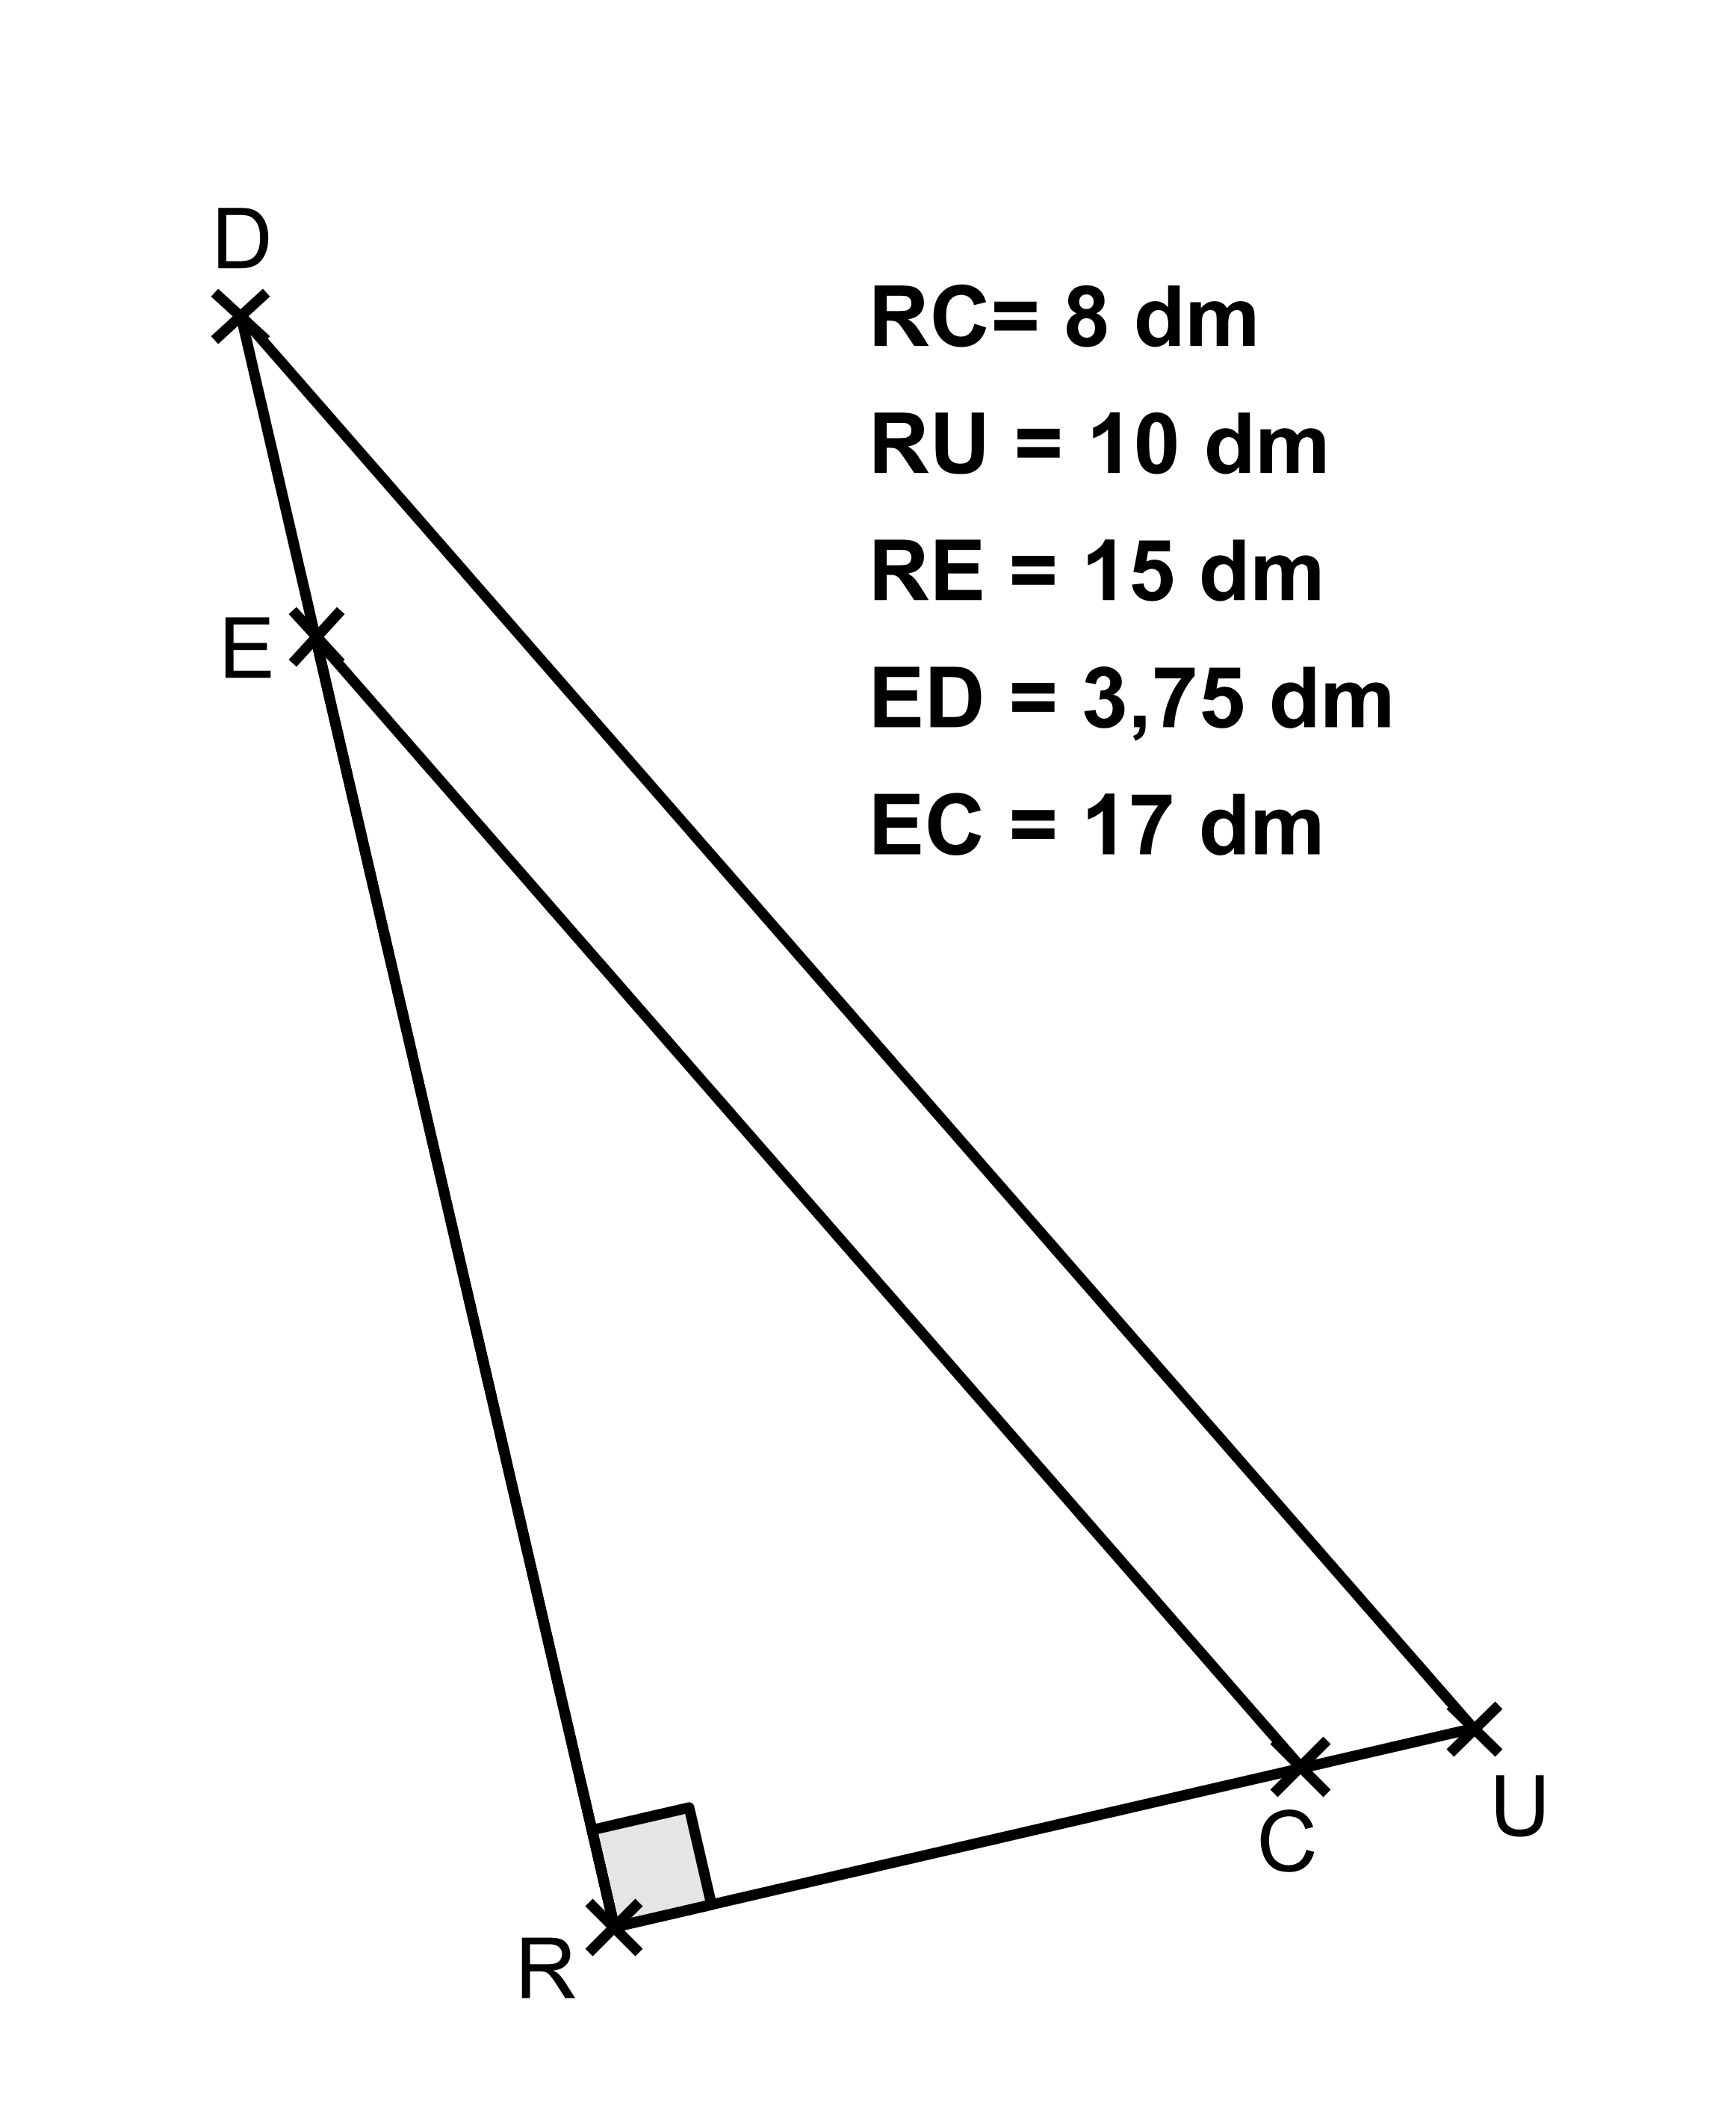
\includegraphics[width=4cm]{images/ex4.png} 
\end{center}
\end{minipage}

\end{tabular}
\end{document}
